\begin{subsubsection}{Power System}
As stated previously, the 2019 mission requirements for distance and time constraints created significant challenges in finding a capable power system. Several weeks of initial design simulation was performed with the online tool ecalc.ch. This allowed the team to quickly simulate a wide number of possible configurations combining motors, electronic speed controls (ESC's), and propellers. Several configurations were found that meet the distance requirement but it wasn’t until the team looked at fixed wing propellers (mounted on higher speed motors) that a viable configuration was found. The high pitch of fixed wing propellers, slightly higher Kv motors, and a higher voltage power system, allowed the multirotor to sustain thrust at high speed. Once this characteristic was identified the available propellers were quickly limited to the 20x13" from APC Propellers as no other comparable propeller was found. This paired with a motor in the 150-200kv range operating at 50v (12s LiPo) provided the necessary thrust. A final configuration using 22Ah of battery and a choice of two motors and ESCs satisfied all of the mission’s requirements in simulation. 

The APC 20x13” props were placed on a dynamometer for validation of specifications and curve fitting RPM to thrust values. UBC UAS tests showed the propeller performing at or above the data supplied by APC and thus met the team’s needs for the mission. Mapping RPM to thrust allowed testing at higher thrust levels as the team’s dynamometer was limited to 5kg, while measuring of higher RPM values was simply measuring the ESC output frequency with a conversion factor. 

\vspace{5mm}
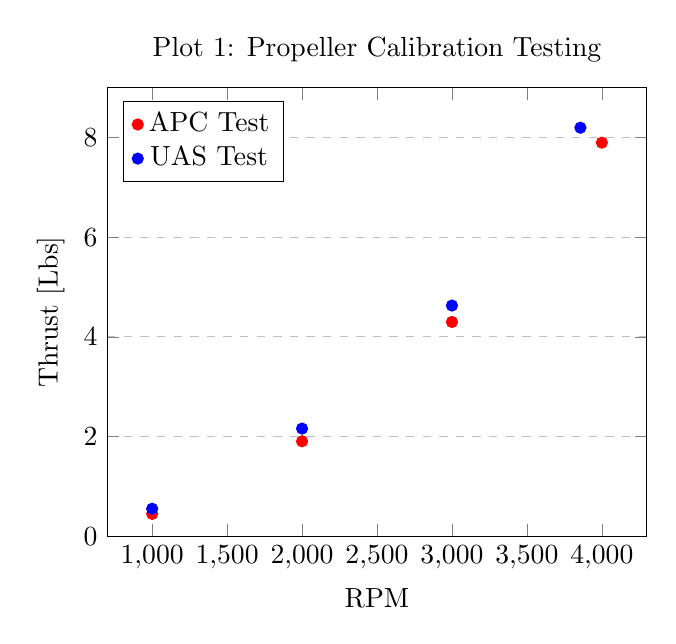
\begin{tikzpicture}
\label{Fig:propeller_calibration_testing}
\begin{axis}[
    title={Plot 1: Propeller Calibration Testing},
    xlabel={RPM},
    ylabel={Thrust [Lbs]},
    %xmin=0, xmax=100,
    ymin=0, ymax=9,
    %xtick={0,20,40,60,80,100},
    %ytick={0,20,40,60,80,100,120},
    legend pos=north west,
    ymajorgrids=true,
    grid style=dashed,
]
\addplot[only marks, color=red]
    coordinates {
    (1000,0.447)(2000,1.905)(3000,4.3)(4000,7.9)};
\addplot[only marks, color=blue]
    coordinates {
    (1000,0.551)(2000,2.16)(3000,4.63)(3857,8.2)};
\legend{APC Test,UAS Test}
\end{axis}
\end{tikzpicture}

\paragraph{Testing}
Final motor and ESC decisions required bench testing of components. One of each T-motor (MN601s-170kv and MN605s-170kv) motor was tested along with both the traditional T-motor Flame 60A HV and the newer Alpha 60A HV FOC (Field Oriented Control) ESCs. Both ESCs were tested for response time and efficiency in terms of thrust per watt of input power (See Plot 2: ESC Efficiency Testing). While there was not a significant difference in either of these metrics the Alpha ESCs were chosen because of their data logging capabilities and over power limiter. This over power limit is important as bench calculations showed the possibility of drastically overpowering the motors at the very top of the throttle curve. 

    % \begin{figure*}\centering
    % \includegraphics[width=0.9\textwidth]{table/table_1.png}
    % \caption*{}
    % \label{fig:msa}
    % \end{figure*}


\vspace{5mm}
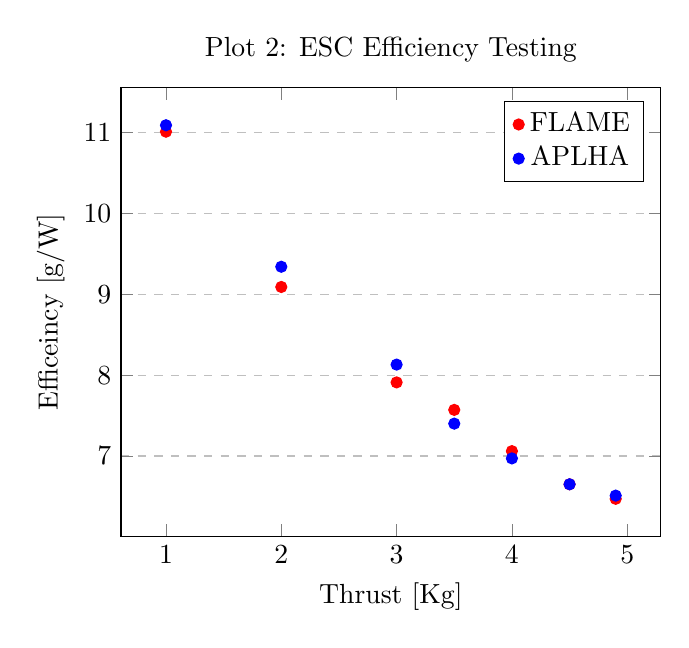
\begin{tikzpicture}
\begin{axis}[
    title={Plot 2: ESC Efficiency Testing},
    xlabel={Thrust [Kg]},
    ylabel={Efficeincy [g/W]},
    %xmin=0, xmax=5,
    %ymin=0, ymax=9,
    legend pos=north east,
    ymajorgrids=true,
    grid style=dashed,
]
\addplot[only marks, color=red]
    coordinates {
    (1,11.01)(2,9.09)(3,7.91)(3.5,7.57)(4,7.06)(4.5,6.65)(4.9,6.47)};
\addplot[only marks, color=blue]
    coordinates {
    (1,11.09)(2,9.34)(3,8.13)(3.5,7.40)(4,6.97)(4.5,6.65)(4.9,6.51)};
\legend{FLAME,APLHA}
\end{axis}

\end{tikzpicture}

Both motors from T-Motor were also tested for total available thrust and power consumption at cruise thrust. Cruise thrust was calculated as a function weight and speed with simplified drag equations. It was found that the increased weight and power consumption of the MN605s projected to reduce the flight time by less than a minute. The additional power of the MN605s was deemed to be desirable as it improved controllability, and there was some uncertainty in exact final all up weight for the aircraft.  

\subsubsection{Frame}
In order to accommodate such a heavy aircraft and power system, a strong and more importantly, stiff frame was required. From previous experience, the team found that a frame that is not sufficiently able to deal with vibrations can prove to be near impossible to tune for stable flight. This led the team to opt for significantly larger frame tubes than have been used in the past at 30mm diameter. Additionally the arms were shortened as much as possible. The center plates, forming a standard “sandwich” design, were constructed out of $1/4$” aluminum - water jetted to remove all extraneous material and weight.  The center plate was also made as small as possible in overall dimensions to reduce bending moments. The simple and classic sandwich design uses very few unique parts making it very quick to assemble as easy to keep spare parts on hand.  

A strong separation was made between payload systems and flight systems on the aircraft, for the purpose of modularity. This meant a completely separate removable center plate for payload systems that sits under the aircraft and is secured with 4 bolts and a single multi-pin cable. This configuration offers significant benefits in parallel development efforts, as well as the ability to quickly switch out payloads as will be necessary for UBC UAS’ second Canadian competition in May that requires a completely different payload. 

Refer to Figure 1 for airframe dimensions.

\begin{center}
\begin{tabular}{c c c } 
 \hline
 Property & Metric & Imperial \\ 
 \hline
 Overall Width & 1508mm & 59in \\ 
 Overall Width (w/o Props) & 1000mm & 39in \\ 
 Maximum Takeoff Weight & 11.5 kg & 25 lbs \\
 Cruise Speed & 12 m/s  & 21 knots \\
 Maximum Speed & 25 m/s & 49 knots \\
 Operational Range & 11.3 km & 7 Miles \\
 Max Flight Time & \multicolumn{2}{c}{30 min} \\
 Batteries & \multicolumn{2}{c}{16-24 Ah, 12S batteries} \\
 Total Power capacity & \multicolumn{2}{c}{1020Wh} \\
\end{tabular}
\end{center}

\begin{figure}[ht]\centering
\includegraphics[width=\linewidth]{figures/Frame}
\caption{Frame}
\label{fig:frame}
\end{figure}


\end{subsubsection}

\endinput